\begin{figure}[h]
    \centering
    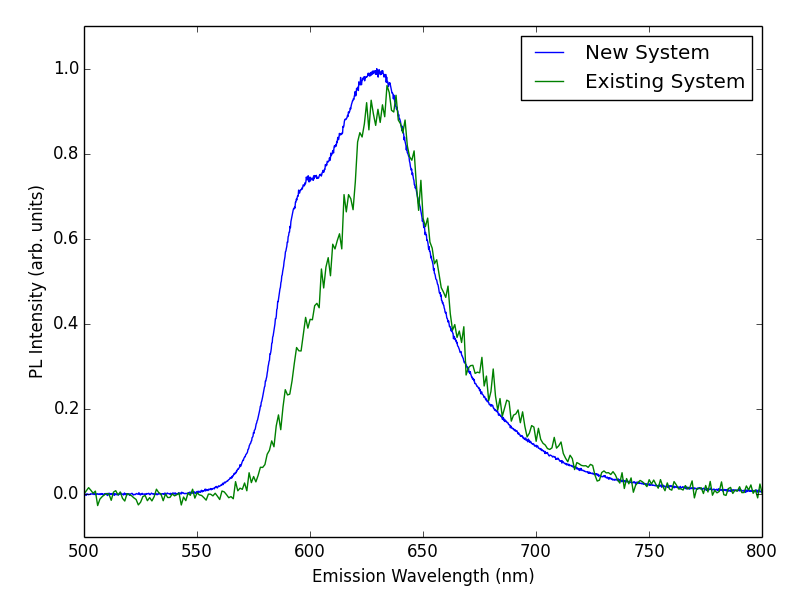
\includegraphics[width=\textwidth]{./img/tesf-2.png}
    \caption{Emission spectrum of ADT TES-F, excited at 405nm.
    Wide-field illumination used by the existing system to excite the sample
    yields a noisy spectrum, and does not excite the secondary peak that is 
    shown clearly in the results from the new system. This may be because the
    wide-field illumination is exciting many adjacent crystals in the sample, 
    which emit slightly different spectra. The laser illumination in the new 
    system has the spatial resolution necessary to illuminate single crystals.}
    \label{fig:pl-adt-tesf}
\end{figure}

\begin{figure}[h]
    \centering
    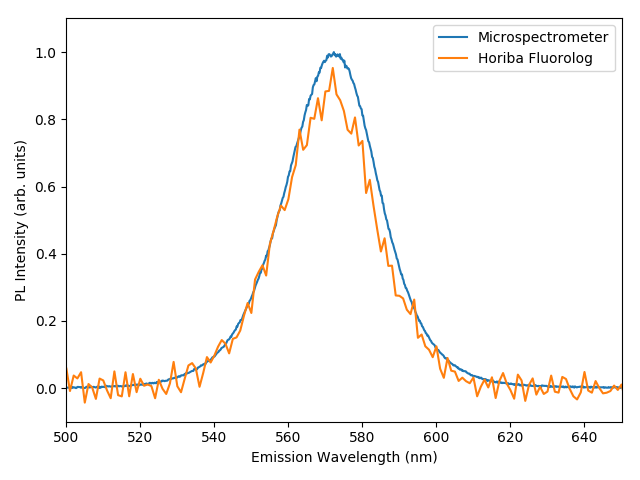
\includegraphics[width=\textwidth]{./img/qd-2.png}
    \caption{PL spectra for CdSe quantum dots in solution, as measured by the new system vs. the existing fluorimeter system.}
    \label{fig:pl-adt-qd}
\end{figure}